\section{A Primer on Atoms, Nuclei, and Isotopes}
\label{appendix_nuclear_primer}
%By Matt Trawick

{\setlength{\baselineskip}{1.15\baselineskip} \setlength{\parskip}{1.5 \parskip}
\bigskip
\textbf{Structure of Atoms}

Atoms are made of positively charged \textit{protons}, negatively charged \textit{electrons}, and uncharged or neutral \textit{neutrons}.  The protons and neutrons are found together in the atom's dense, central \textit{nucleus}, while the 
electrons are 
\begin{wrapfigure}[10]{r!}{0.32 \textwidth}
\begin{center}
\vspace{-0.2in}
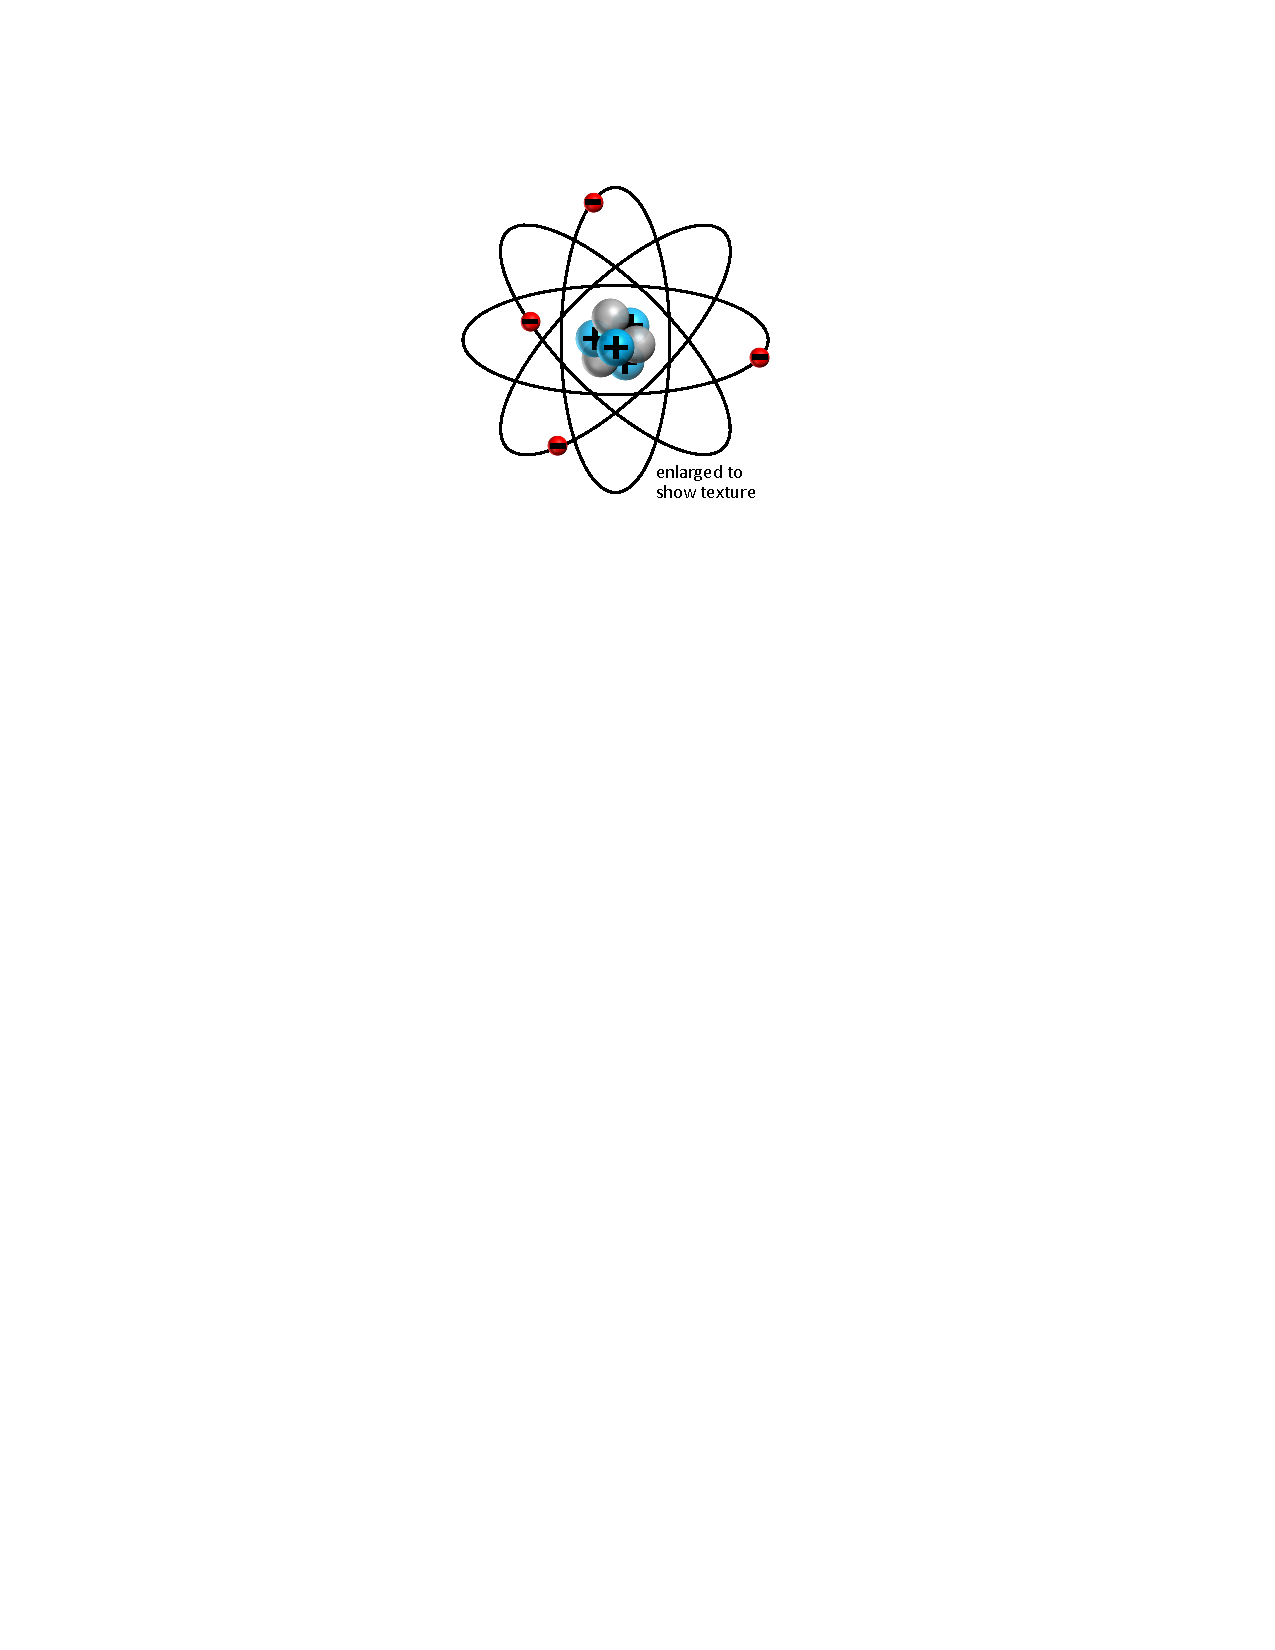
\includegraphics[scale=0.85]{appendices/atom_figure.pdf}
\index{color page}
\end{center}
\end{wrapfigure}
distributed outside the nucleus.  Although common depictions of atoms (like that on the right) show the electrons as well-defined little balls in distinct orbits, a more realistic model would be more like a fuzzy cloud, in which individual electrons have neither a finite size nor well-defined locations.

\medskip

\textbf{Elements, Isotopes, and Nuclear Notation}

The number of protons in an atom (its ``atomic number'') determines which element it is and is responsible for all of its chemical properties.  (The number of electrons is generally the same as the number of protons, though it is possible for an atom to lose or gain an electron if it becomes ionized.)  By contrast, the number of neutrons can vary slightly among atoms of the same element, with each number of neutrons defining a different \textit{isotope} of that element.  For example, all chlorine nuclei contain 17 protons (that's what makes them chlorine atoms), but can be commonly found in nature with either 17 or 19 neutrons.  These two isotopes of chlorine are mostly indistinguishable except for their mass:  
their \textit{atomic mass numbers} 
are 34 and 36, respectively, obtained by adding the number of protons plus the number of neutrons.  
%The natural abundances of the two isotopes are 76\% and 24\%, so the average atomic mass of chlorine found in nature works out to about 34.45 atomic mass units (amu).
Isotopes are named by their atomic mass numbers, e.g. chlorine-34 or chlorine-36.
(Note: all lowercase and hyphenated.)
%(The element name is not capitalized, and there's a hyphen before the mass number.)



{\setlength{\baselineskip}{1.1 \baselineskip}

\begin{wrapfigure}[7]{l}{0.28 \textwidth}
\begin{center}
\vspace{-0.35in}
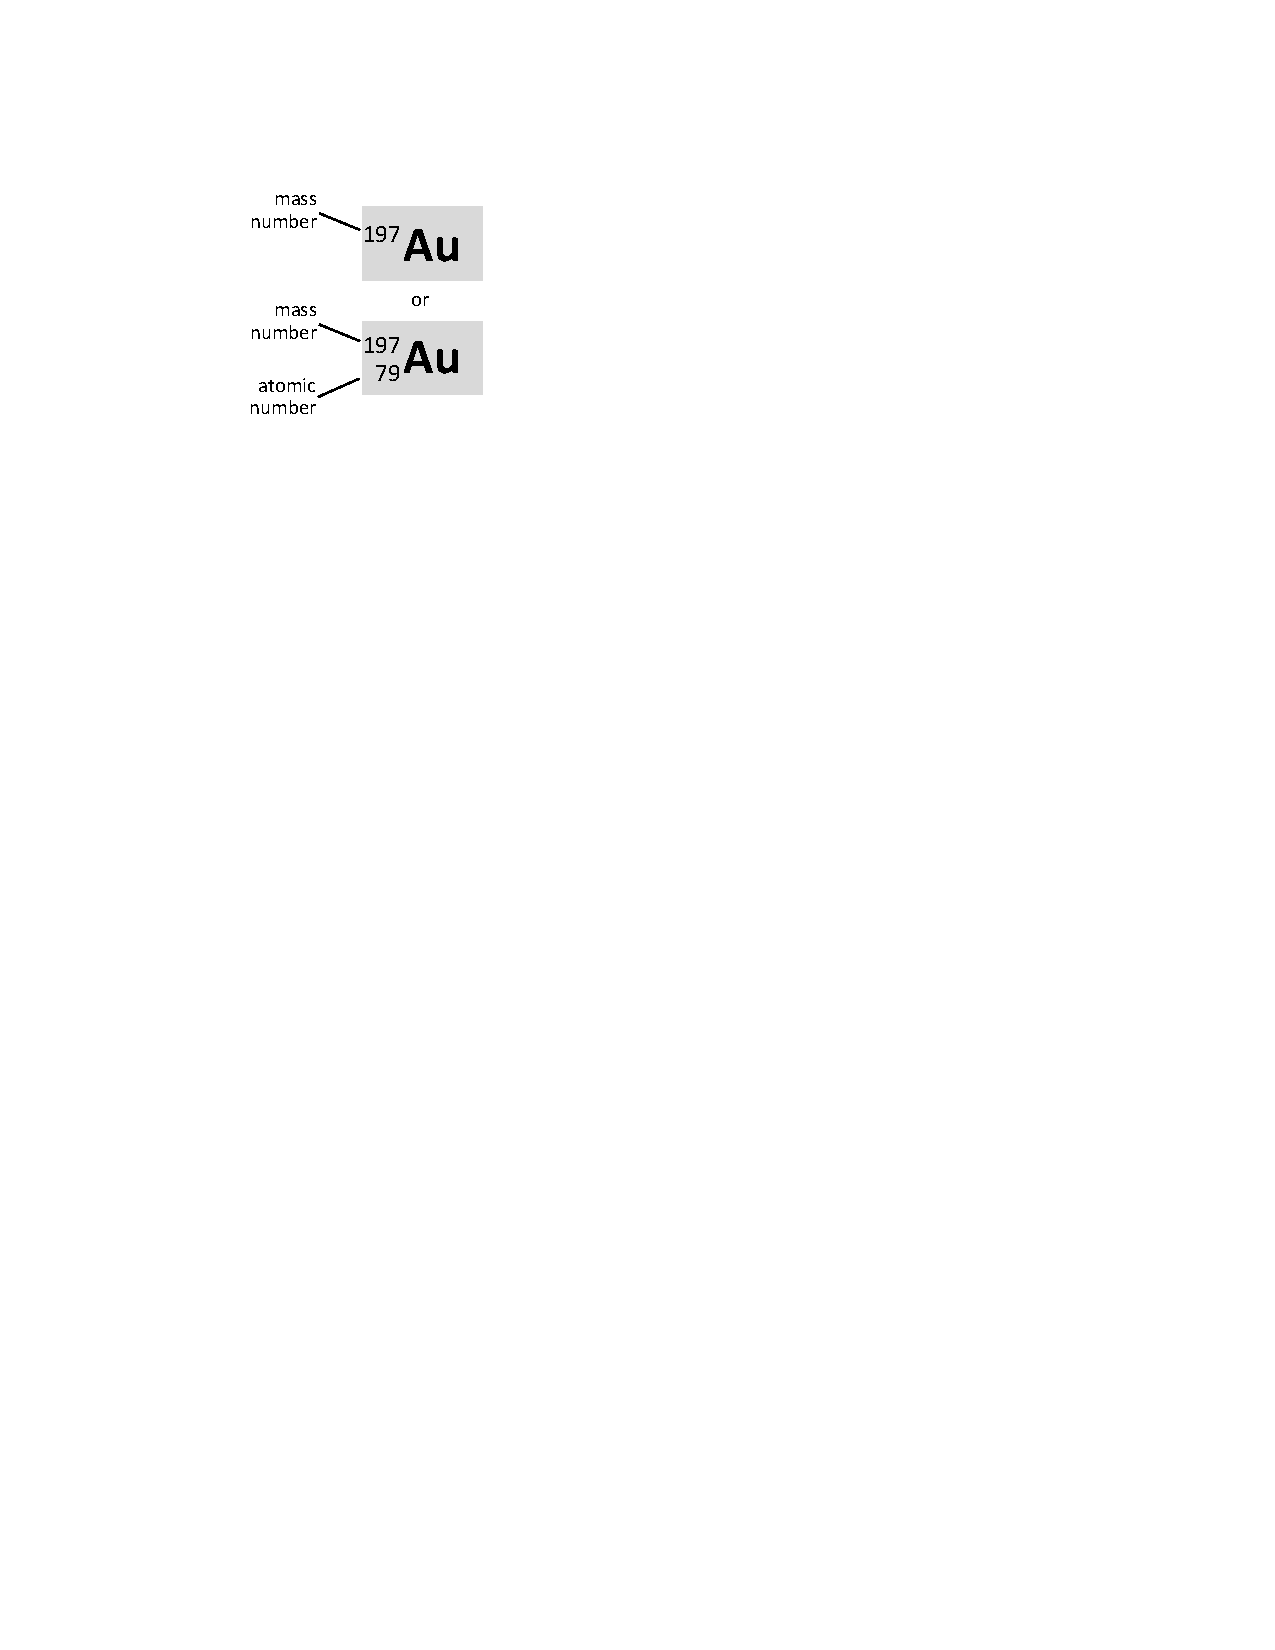
\includegraphics[scale=0.85]{appendices/isotope_abbreviations.pdf}
\end{center}
\end{wrapfigure}
To abbreviate an isotope, we write the atomic mass number as a superscript before the element's standard chemical symbol (Cl for chlorine, O for oxygen, etc.), as in \isotope[34]{Cl} and \isotope[36]{Cl} (read as ``chlorine-thirty-four'' and ``chlorine-thirty-six'').
When writing for non-experts, one can also (optionally) include the atomic number 
%in the abbreviation, written as a subscript 
below the mass number: \isotope[34][17]{Cl} and \isotope[36][17]{Cl}.  
%(The number of neutrons can be found by subtracting the two given numbers, i.e. ($36 - 17 = 19$~neutrons in the latter case.)  
Technically, the atomic number is redundant, giving no additional information beyond the atomic symbol---but only provided that the reader has memorized the entire period table.

} %end of increased baselineskip

\textbf{Sizes and Masses}

The radii of atoms range in size from $\approx 3 \times 10^{-11}$ to $\approx 3 \times 10^{-10}$ meters.  Atomic \textit{nuclei} are even smaller, with radii ranging from $\approx 1 \times 10^{-15}$ meters for hydrogen (a single proton) to $\approx 6 \times 10^{-15}$ meters for uranium.\footnote{There's quite a bit of slop in all of these sizes, in part because the outer boundary of an atom or nucleus is not well-defined.  For both atoms and nuclei, the distribution of mass and electrical charge has fuzzy edges rather than sharp cut-offs; different definitions and different measurements thus yield varying figures.}
Most of the mass of an atom is in its nucleus; protons and neutrons both have masses of roughly 1~amu, or $1.66\times 10^{-27}$~kg.  An electron has a much smaller mass, about $\frac{1}{1823}$~amu, or $9.11\times 10^{-31}$~kg---yet it's the electrons in an atom that take up most of the space.  
%It's hard to appreciate just how dense an atomic nucleus is, but one useful example is a ``neutron star'', in which a star at the end of its normal life cycle collapses into pure, compressed nuclear matter, roughly the same density as an atomic nucleus.  A neutron star has roughly the mass of our own Sun, but a diameter of only about 20 kilometers.  
For some perspective, a teaspoon of matter with the same density as an atomic nucleus would have a mass of $\approx 10^{11}$~kg, about the same as the mass of a 1-km-high mountain.  

} %end of increased baselineskip
